\section{Result 3}
Building on the Result 1 analysis, an additional entity - Sakai presence events - was taken into account, requiring configuration adjustments of nETL and CouchDB to aggregate across three entities instead of two entities. This analysis looks at the relationship between student benchmarks in the FU data and resultant course grades as a factor of Sakai usage. In other words, this analysis addresses the question of whether making more frequent use of the Sakai platform is shown to increase course performance for CSC1015F. However, the Sakai data - measured as presence events - cannot be associated with particular courses. As such the analysis takes into account only ``general usage'' of the Sakai LMS, and not usage of Sakai for these particular courses.

The nETL task configurations to load Grade data and FU data into CouchDB are mostly the same as the task configurations as used to achieve Result 1, except that Grade data is filtered to only include course results from 2016 via whitelisting (since Event data is only for 2016). A 3rd task is added to the configuration object to load the Event data into CouchDB. Configuration for nETL and CouchDB Map and List functions is included in the appendix (see \ref{netl-run3-config}, \ref{result-3-map} and \ref{result-3-list} respectively).

\subsection*{\textit{nETL} Event data configuration}
\begin{itemize}
    \item Batches of 30 000 lines are extracted iteratively (and sequentially) as an array of lines (30 000 lines per batch seemed to be the sweetspot for what could be loaded into CouchDB's \textit{\_bulk\_docs} endpoint using nETL and still receiving optimal visual feedback in terms of continuous logging)
    \item Within each batch, each line is converted to a JSON object, transforming the batch into an array of objects. These objects each have the following fields: ``event\_date'', ``event\_id'', ``uct\_id'',  ``site\_key'', ``ref''
    \item The array of objects is filtered via whitelising objects on two fields: 1) ``uct\_id'' - only IDs of students who attended CSC1015F are considered. 2) ``event\_id'' - only the value ``281'' is considered, as these are representative of `presence' events
    \item A field is added to each object in the batch (``type\_'') and give the value ``vulaEvent''
    \item Superfluous object fields are removed via a whitelisting process, resulting in a batch (an array) of objects with the fields: ``event\_date'', ``event\_id'', ``uct\_id'', ``site\_key'', ``type\_''
    \item Each batch is loaded into CouchDB using the \textit{\_bulk\_docs} endpoint (as discussed previously), and the next batch is extracted on a success message from CouchDB
\end{itemize}

\subsection*{The MapReduce function}
Compared to the function logic illustrated in \ref{result-1-map-fn}, an additional logical branch is required to handle Event data. This is shown in \ref{result-3-map-fn}.

\begin{figure}[ht]
    \centering
    \begin{mdframed}
        \centering
        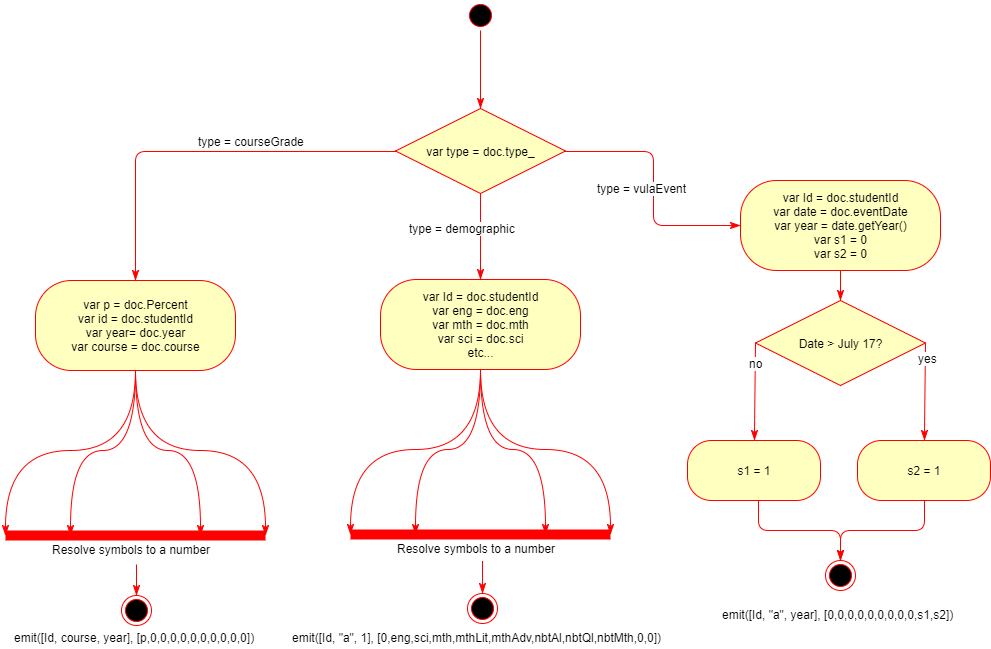
\includegraphics[scale=0.35]{./resources/figures/activity-diagram-2.png}
    \end{mdframed}
    \caption[Result 1 Map function]{\textbf{Figure \ref{result-3-map-fn}: Activity diagram showing logic Map function logic for Results 3 \& 4.} The map function comprises a decision tree with 3 logical branches depending on the type of document: FU documents are logically treated as according to the left branch, grade document the center branch, and Sakai event document as according to the logic depicted in the right hand branch. During index calculation each document is processed as according to this decision tree, with a slightly different key:value pair emitted depending on the type of document being processed - although the structure of the emitted key:value pair is identical for all document types. For documents of type 'grade', the key consists of the tuple [Id, Grade, year], the values of which are derived from the document being processed. For documents of type 'demographic', the key is a tuple that consists of the form [Id, ``a'', 2016], and for `event' documents the key emitted is of the form [Id, `a', year]. Since documents of type `event' and `demographic' do not include course information the value `a' is emitted. Similarly, for documents of type `demographic', there is no year field. So the value of `1' is always emitted. Emitting hard coded values allows for grouping documents by student Ids together and guarantees that documents of different types but with the same student Id are treated sequentially due to the nature of the b+tree storage engine. As such, aggregating different entity types across the same student Id is possible during index reading and doesn't require processing of data in addition to the retrieval process. Depending on the logical branch traversed during map function execution, different indexes of the value tuple are populated; by default this tuple instantiated on every map function execution as a list of 11 zeros. The map function then alters the value at different indexes for different document types. If the document being processed is a 'grade' document, the value at index = 0 is adjusted to be the grade percent. For 'demographic' documents, the values at indexes 1 through 8 are adjusted. And for 'event' documents, the map function adjusts values at indexes 9 and 10 before emitting the key:value pair. Since the value tuple }
    \label{result-3-map-fn}
\end{figure}

\subsection*{The List function}
Compared to the List function used to translate the index JSON output to CSV output, minor changes are implemented to handle the two additional fields in the values of the map function output. The function is included in the appendix for reference (see \ref{result-3-list})